\documentclass[a4paper, 12pt, titlepage]{article}
\usepackage{ctex} 
\usepackage{amssymb}
\usepackage{amsmath}
\newtheorem{theorem}{Theorem}
\newtheorem{lemma}{Lemma}
\newtheorem{proof}{Proof}

\usepackage[noend]{algpseudocode}
\usepackage{algorithmicx,algorithm}
\renewcommand{\algorithmicrequire}{\textbf{Input:}}
\renewcommand{\algorithmicensure}{\textbf{Output:}}

\usepackage{mathtools}

\usepackage{graphicx}

\usepackage{indentfirst}
\setlength{\parindent}{2em}
\usepackage[CJKbookmarks]{hyperref}

\usepackage{enumerate}

\usepackage{listings}
\usepackage{latexalpha2}

\begin{document}

% \begin{CJK}{UTF8}{gbsn}
\title{Problem Set 3 Solutions}
\author{姓名: 黄睿 \\ 学号: MP1933008}
\date{2019-11-16}


\maketitle
% \end{CJK}

\section{Problem 1}

\subsection{Q1}
\begin{algorithm}[h]
    \caption{Greedy algorithm for max $k$-cut}
    \begin{algorithmic}[1]
        \Require {\bf G(V,E)}
        \Ensure {$S_1, S_2, \cdots, S_{k}$}
        \State Init $S = \{S_1, S_2, \cdots, S_{|V|} \}$ with $S_{i} = \{ v_{i} \}, i = 1, 2, \cdots, |V| $;
        \While{$|S| \geq k$}
 			\State pick $S_{i}$ and $S_{j}$ with edges between them have {\bf smallest weight},  contract $S_{i}$ and $S_{j}$ into $S_{\min{(i, j)}}$.
        \EndWhile
        \State \Return $S_1, S_2, \cdots, S_{k}$
    \end{algorithmic}
\end{algorithm}

To analyze the approximation ratio, we define that on each contraction the weight of edges is $W_{i}, i= 1, 2, \cdots, |V|-k$.As we take the greedy strategy, it's obvious that there is monitonicity, shows that: $W_{1} \leq W_{2} \leq \cdots \leq W_{|V| - k}$, we also have:
\begin{equation}
	\begin{aligned}
		W_i &\leq \frac{\sum_{e \in E} W_e - \sum_{j = 1}^{i - 1} W_{j}}{\binom{|V| - i + 1}{2}} \\
			&\leq \frac{\sum_{e \in E} W_e - (i - 1) W_i}{\binom{|V| - i + 1}{2}} \\
	\end{aligned}
\end{equation}
simplify the inequality above:
\[
	W_i \leq \frac{2 \sum_{e \in E} W_{e}}{(|V| - i)(|V| -i + 1)}
\]
the term on the right side is the average weight, and we can make it sure that:$OPT \leq \sum_{e \in E} W_{e}$.

The greedy algorithm will produce:
\begin{equation}
	\begin{aligned}
		SOL &= \sum_{e \in E} W_{e} - \sum_{i = 1}^{|V| - k} W_{i} \\
			&\geq \sum_{e \in E} W_{e} - \sum_{i = 1}^{|V| - k} \frac{2 \sum_{e \in E} W_{e} }{(|V| - i)(|V| -i + 1)} \\
			&= \sum_{e \in E} W_{e} \left[1 - 2 \sum_{i = 1}^{|V| - k} \left( \frac{1}{|V| - i} - \frac{1}{|V| - i + 1} \right) \right] \\
			&= \sum_{e \in E} W_{e} \left[1 - 2 \left(\frac{1}{k} - \frac{1}{|V|} \right) \right] \\
			&\geq \left[ 1 - 2 \left(\frac{1}{k} - \frac{1}{|V|} \right) \right] \cdot OPT
	\end{aligned}	
\end{equation}
	
\subsection{Q2}
The missing code:
\underline{move $v$ to $S_{1-i}$ will yield a larger weighted cut};

The time complexity of this algorithm is : $O(|V|^2 \sum_{e \in E} w_e)$, for each round of the while loop involves examining at most $|V|$ vertices and selecting one that increases the cut
value when moved.This process takes $O(|V|^2)$ time. Since we assume that edges have positive integral weights, the cut value is increased by at least 1 after each iteration.The maximum
possible cut value is $\sum_{e \in E} w_e$.Combining all of them, we get the total running time: $O(|V|^2 \sum_{e \in E} w_e)$.

To analyze the approximation ratio, we first notice that for any max 2-cut:
\[
    w(S_0, S_1) = \sum_{uv \in E \atop u \in S_0, v \in S_1} w(uv) \leq OPT \leq \sum_{e \in E} w(e) 
\]
According to the local search algorithm, it will end with: for any $u \in S_0$, moving $u$ to $S_1$ will not increase the cut value, thus:
\[
    \sum_{u \in S_0 \atop uv \in E} w(uv) \geq  \sum_{u \in S_1 \atop uv \in E} w(uv) 
\]

\begin{equation}\label{eq:eq1}
    2 \sum_{u \in S_0 \atop uv \in E} w(uv) \geq \sum_{u \in S_0 \atop uv \in E} w(uv) + \sum_{u \in S_1 \atop uv \in E} w(uv) = \sum_{u: uv \in E} w(uv)
\end{equation}
By symmetry, we have:
\begin{equation}\label{eq:eq2}
    2 \sum_{v \in S_1 \atop uv \in E} w(uv) \geq  \sum_{v: uv \in E} w(uv)
\end{equation}

Combining \ref{eq:eq1} and \ref{eq:eq2}, we have:
\begin{equation}
    \begin{aligned}
        w(S_0, S_1) &= \left( \sum_{u \in S_0 \atop uv \in E} w(uv) + \sum_{v \in S_1 \atop uv \in E} w(uv) \right) \\
                    &\geq 0.5 \cdot \sum_{e \in E} w(e) \\
                    &\geq 0.5 \cdot OPT
    \end{aligned}
\end{equation}
Thus, we proved the approximation ratio is $0.5$.
\section{Problem 2}
\begin{algorithm}[h]
    \caption{Greedy algorithm for max $k$ coverage}
    \begin{algorithmic}[1]
        \Require {$S_{1}, S_{2}, \cdots, S_{m}$}
        \Ensure {C}
        \State Init $C = \emptyset$;
        \While{$|C| < k$}
 			\State add $i$ with largest $|S_{i} \cap U|$ to $C$;
 			\State $U = U \backslash S_{i}$;
        \EndWhile
        \State \Return $C$
    \end{algorithmic}
\end{algorithm}

Let $C_{i}$ be the elements covered in $i$ coverage, where $i = 1, 2, \cdots, k$.We can prove the approximation ratio by performing induction on $i$.

If $i = 1$, It's trivial that: $C_{1} \geq 1 - \left( 1 - \frac{1}{k} \right)^{1} \cdot OPT$.
By taking greedy strategy we have each step, we cover \textbf{at least} $\frac{1}{k}$ of uncovered elements.Thus,
\begin{equation}
	\begin{aligned}
		C_{i + 1} &\geq C_{i} + \frac{OPT - C_{i}}{k - i} \\
				  &\geq \left(1 - \frac{1}{k} \right) C_{i} + \frac{OPT}{k} \\
				  &\geq \left(1 - \frac{1}{k} \right)\left[ 1 - \left( 1 - \frac{1}{k} \right)^{i} \right] \cdot OPT + \frac{OPT}{k} \\
				  &\geq \left[ 1 - \left( 1- \frac{1}{k} \right)^{i + 1} \right] \cdot OPT
	\end{aligned}
\end{equation}
Let $i + 1 = k$, we have:
\[
	C_{k} \geq \left[ 1 - \left( 1 - \frac{1}{k} \right)^{k} \right] \cdot OPT
\]

\section{Problem 3}

\subsection{Q1}
The expected size of random cut is given by:
\begin{equation}
	\begin{aligned}
		\mathbb{E} \left[ | E(S,T)|\right] &= \sum_{(u,v) \in E} \Pr \left[ u \in S, v \in T \right] \\
			&= \sum_{(u,v) \in E} \Pr \left[u \in S \right] \cdot \Pr \left[ v \in T \right] \\
			&= \sum_{(u,v) \in E} \frac{1}{2} \cdot \frac{1}{2} \\
			&= \frac{1}{4} \cdot OPT
	\end{aligned}
\end{equation}
According to what we have shown above, the approximation of random cut is $\frac{1}{4}$.

\subsection{Q2}
Similar to Q1:
\begin{equation}
	\begin{aligned}
		\mathbb{E} \left[ | E(S,T)|\right] &= \sum_{(u,v) \in E} \Pr \left[ u \in S, v \in T \right] \\
			&= \sum_{(u,v) \in E} \Pr \left[u \in S \right] \cdot \Pr \left[ v \in T \right] \\
			&= \sum_{(u,v) \in E} \left(\frac{1}{4} + \frac{x_{u}^{*}}{2}\right) \cdot \left(1 - \left( \frac{1}{4} + \frac{x_{v}^{*}}{2} \right) \right) \\
			&= \sum_{(u,v) \in E} \left(\frac{1}{4} + \frac{x_{u}^{*}}{2}\right) \cdot \left(\frac{1}{4} + \frac{1 - x_{v}^{*}}{2} \right) \\
			&\geq \sum_{(u,v) \in E} \left( \frac{1}{4} + \frac{ y_{u,v}^{*} }{2} \right)^2 \\
			&= \sum_{(u,v) \in E} \left( \frac{1}{4} - \frac{ y_{u,v}^{*} }{2} \right)^2 + \frac{ y_{u,v}^{*} }{2} \\
			&\geq \sum_{(u,v) \in E} \frac{ y_{u,v}^{*} }{2} \\
			&= \frac{1}{2} \cdot OPT_{LP}
	\end{aligned}
\end{equation}
We have:
\[
	\mathbb{E} \left[ | E(S,T)|\right] \geq \frac{1}{2} \cdot OPT_{LP} \geq \frac{1}{2} OPT
\]
the approximation ratio is expected to be $\frac{1}{2}$.

\section{Problem 4}
\subsection{Q1}
The expected number of satisfied clauses is:
\begin{equation}
	\begin{aligned}
		E \left[ \text{\# of satisfied clauses}\right] &= \sum_{j = 1}^{m} \Pr \left[ C_{j} \text{\ is satisfied} \right] \\
		&= \sum_{j = 1}^{m} \left[ 1 - \prod_{i \in S_{j}^{+} } \left( 1- f(x_{i}^{*}) \right) \cdot \prod_{i \in S_{j}^{-} } f(x_{i}^{*}) \right] \\
		&\geq \sum_{j = 1}^{m} \left[ 1 - \prod_{i \in S_{j}^{+} } 4^{-x_{i}^{*}} \prod_{i \in S_{j}^{-} } 4^{x_{i}^{*} - 1} \right] \\
		&= \sum_{j = 1}^{m} \left[ 1- 4^{ \sum_{i \in S_{j}^{-}} (x_{i}^{*} - 1) - \sum_{i \in S_{j}^{+} } x_{i}^{*} } \right] \\
		&\geq \sum_{j = 1}^{m} \left[ 1 - 4^{- y_{j}^{*}} \right] \\
		&\geq \sum_{j = 1}^{m} \left(1 - \frac{1}{4} \right) y_{j}^{*} \qquad (convexity)\\
		&\geq \frac{3}{4} \cdot OPT
	\end{aligned}
\end{equation}
\subsection{Q2}



\subsection{Q3}
It's not possible.

\section{Problem 5}
\subsection{Q1}
Let $x_{j}^{i} = 1$ if element $j$ in subset $S_{i}$, otherwise $x_{j}^{i} = 0$, let $y_{i} = 1$ if $i \in C$, otherwise $y_{i} = 0$.
The integer program can be modeled as below:
\begin{equation}
	\begin{aligned}
		\text{ minimize } & \sum_{i = 1}^{m} w_{i} \cdot y_{i} \\ 
		\text{ subject to } & \sum_{i = 1}^{m} x_{j}^{i} \geq 1 \\
		& x_{j}^{i} \in\{0,1\}, \quad 1 \leq j \leq n, 1 \leq i \leq m \\
		& y_{i} \in\{0,1\}, \quad 1 \leq i \leq m
	\end{aligned}
\end{equation}
By performing LP relaxation, the integer program transforms to LP:
\begin{equation}
	\begin{aligned}
		\text{ minimize } & \sum_{i = 1}^{m} w_{i} \cdot y_{i} \\ 
		\text{ subject to } & \sum_{i = 1}^{m} x_{j}^{i} \geq 1 \\
		& x_{j}^{i} \in [0,1], \quad 1 \leq j \leq n, 1 \leq i \leq m \\
		& y_{i} \in [0,1], \quad 1 \leq i \leq m
	\end{aligned}
\end{equation}

\subsection{Q2}
\begin{figure} 
    \wolframgraphics[pdf]{Plot3D[Sin[x]Cos[y], {x, -2Pi, 2Pi}, {y, -2Pi, 2Pi}]}{example}
    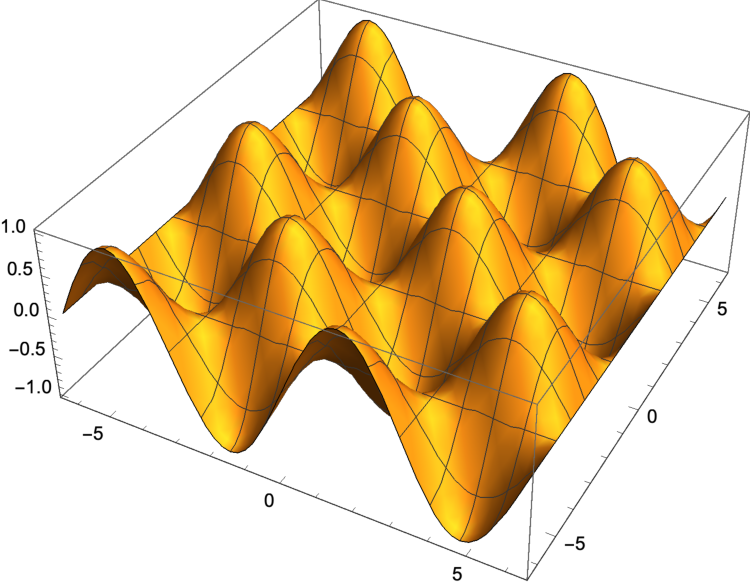
\includegraphics{example.pdf}
    \caption{Plot of $f(x,y)=\sin(x)\cos(y)$}
    \centering
\end{figure}

\begin{figure} 
    \wolframgraphics[pdf]{Table[Plot[{1 - k^(-x), (k - 1)/k x}, {x, 0, 1}], {k, 3, 6}]}{figure2}
    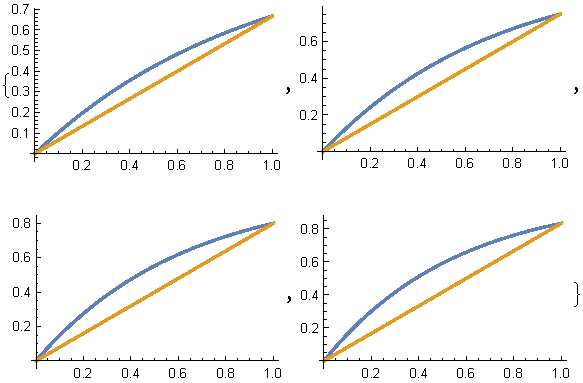
\includegraphics{figure2.pdf}
    \caption{Plot of $f(x) = 1 - \frac{x}{k}$ and $\frac{k - 1}{k} x$}
    \centering
\end{figure}

\end{document}